\subsection{Efficient Encodings}

\label{sec:info_effic}

Now that we are familiar with Binary Tree Encodings (Theorem \ref{theo:binary_tree_encoding}), optimal encodings:
\begin{Def}[Huffman's Algorithm]

    \noindent
    Build a subtree with the two least probable symbols. Such subtree is now 
    considered a single symbol with a probability equal to the sum of the previous two.
    Do so until all symbols are combined into a single tree, called a \textbf{Huffman tree}, an 
    optimal variable-length encoding.

\noindent
\rule{\textwidth}{0.4pt}\\
\textbf{Time Complexity:} $O(n \log n)$, where $n$ is the number of symbols. The actual
encoding is done in $O(n)$ time, the $\log n$ factor comes from the need to sort the symbols by probability.
\end{Def}

\begin{figure}[ht!]
    \centering
    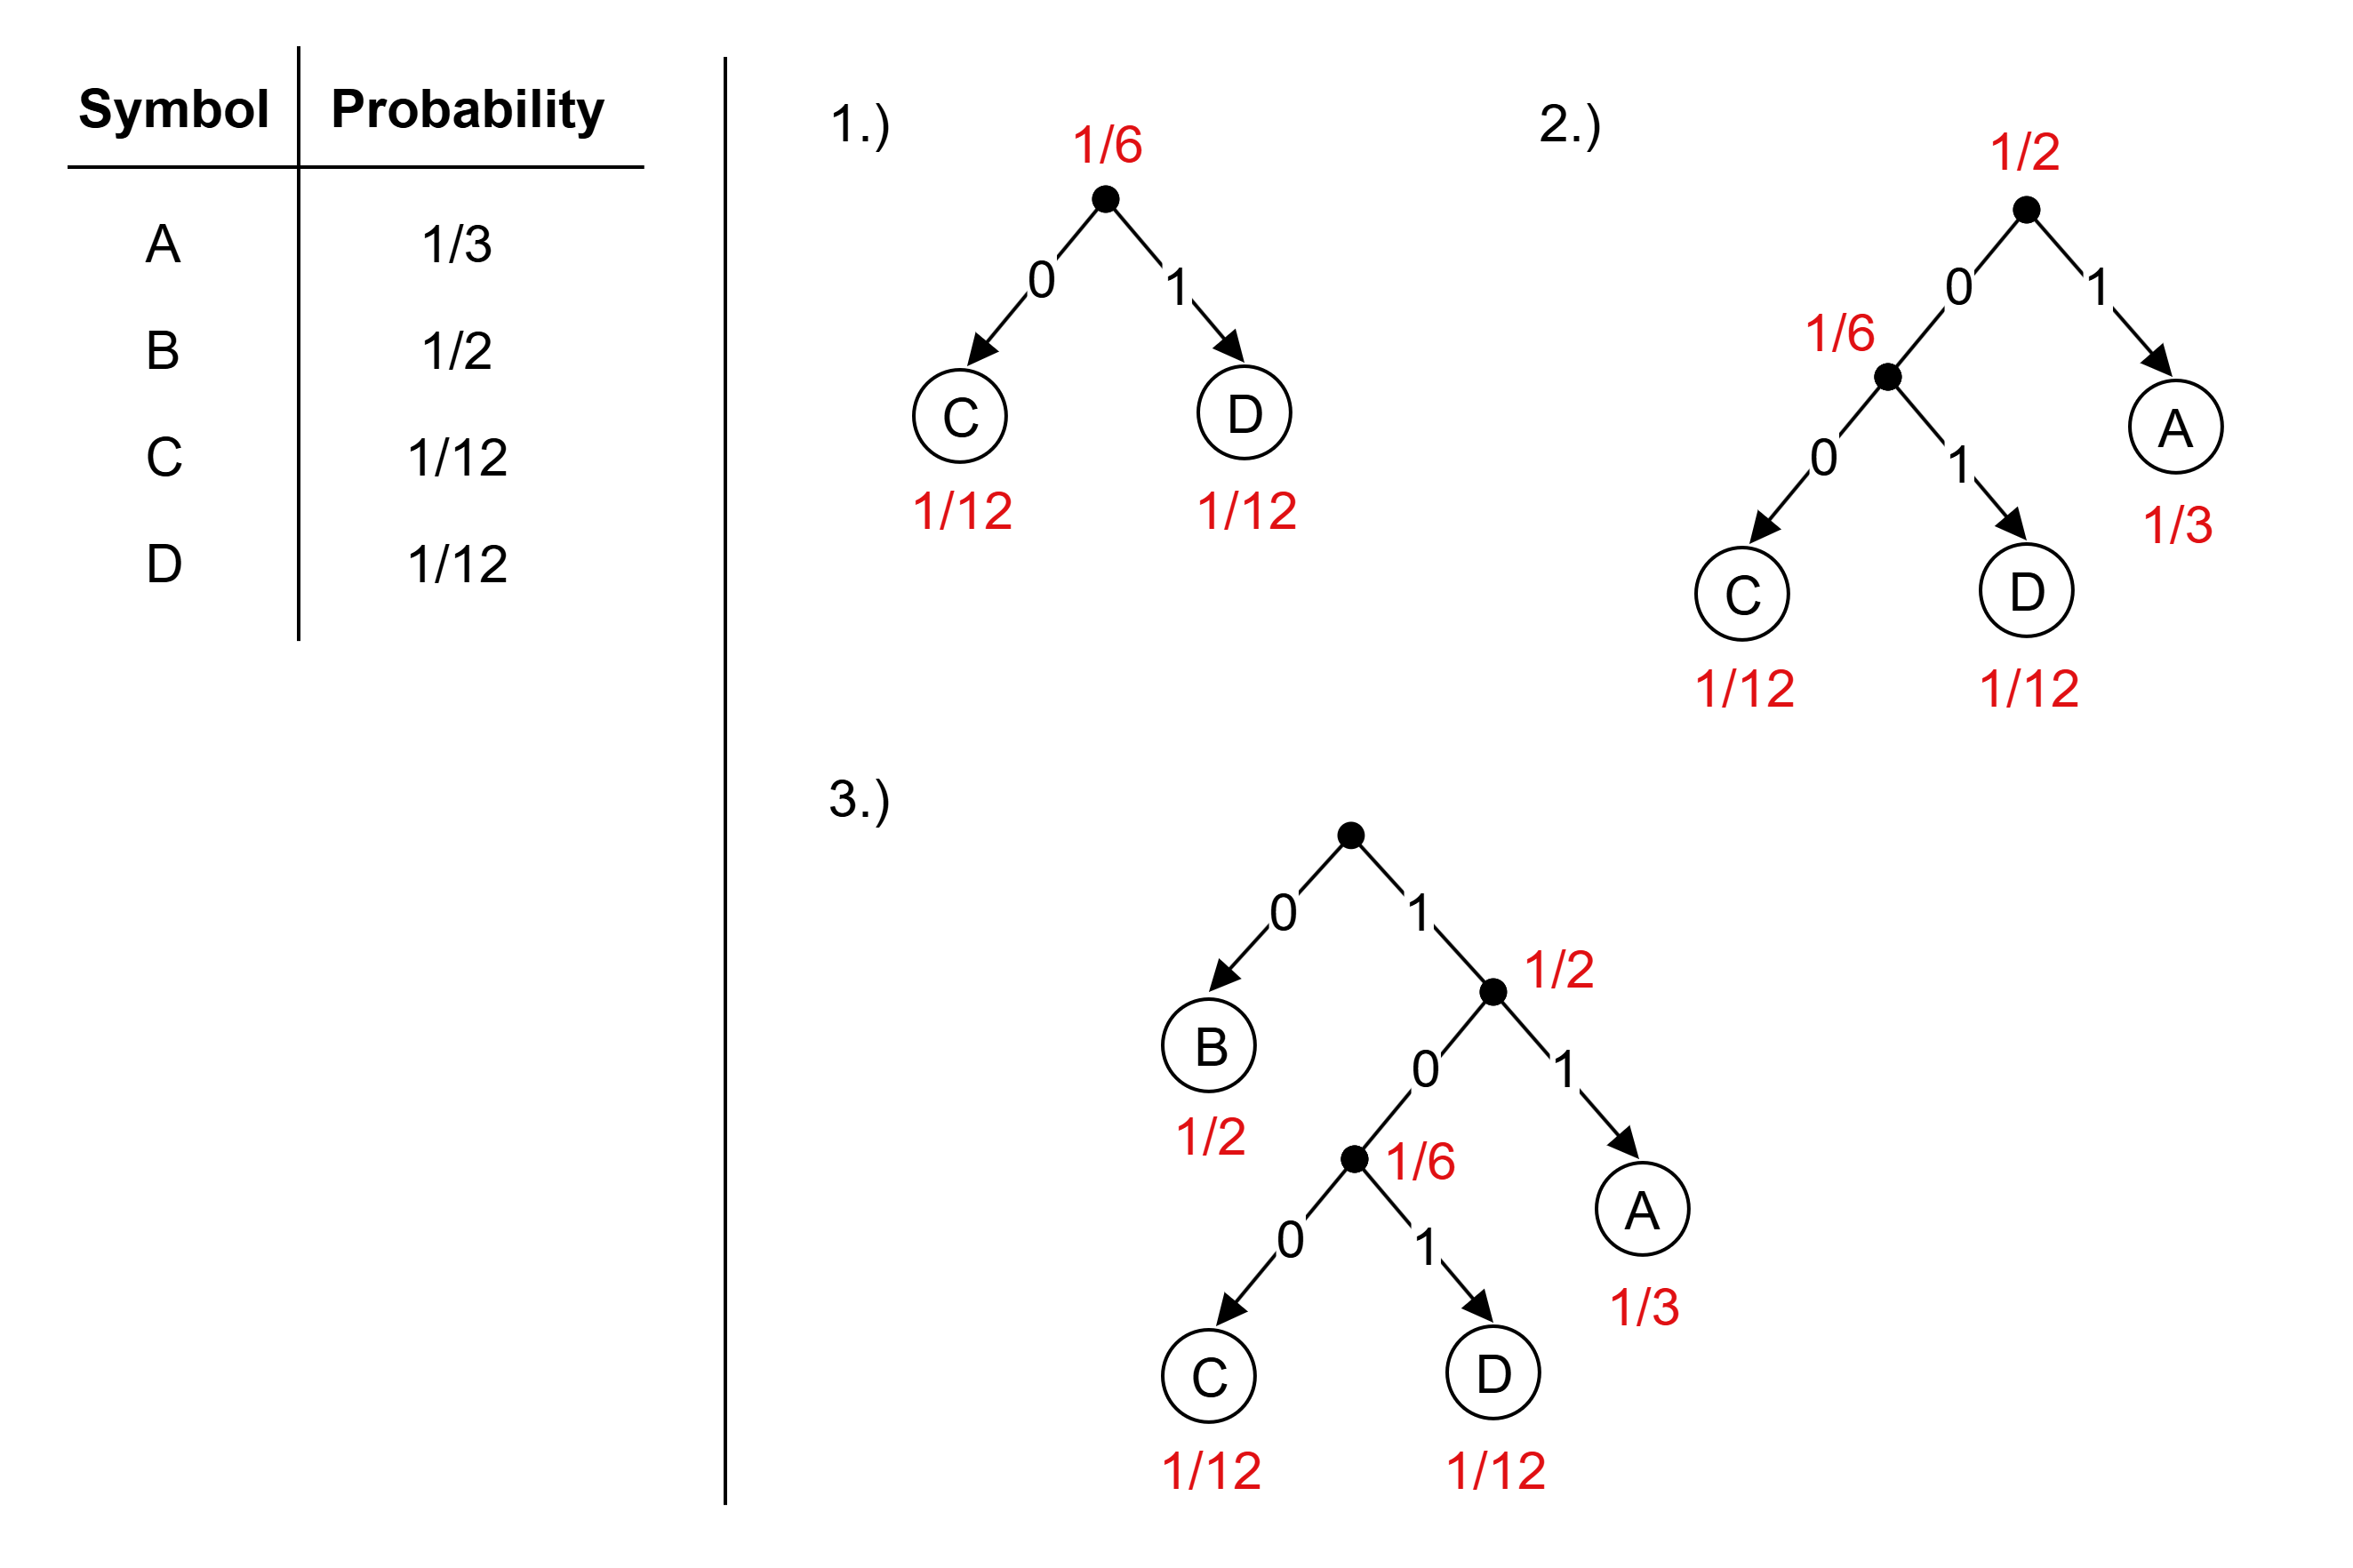
\includegraphics[width=\textwidth]{./Sections/comp/info_effic/huffman_tree.png}
    \caption{A Huffman tree for the symbols $A$, $B$, $C$, and $D$ with their respective probabilities.
    (1) $C$ and $D$ are combined first having the highest probabilities, $1/12$, which combine to a subtree with a probability of $1/6$.
    (2) $A$ is added, $1/3$ combining with the subtree $C+D$ to form a new subtree with a probability of $1/2$.
    (3) Finally, $B$ is added, which has the highest probability of $1/2$, resulting in the final Huffman tree.}
    \label{fig:huffman_tree}
\end{figure}

\newpage 

\noindent
This brings us to the field of compression:
\begin{Def}[Lossless Data Compression]

    \noindent
    Lossless data compression is a technique that reduces the size of a file without losing any information.
    This is often achieved by encoding chunks of redundancy into a single symbol.
\end{Def}


\subsection{Error Detection \& Correction}

\label{sec:info_error}
Two people Alice and Bob were trying to communicate a game of heads or tails over a noisy channel:

\begin{figure}[ht!]
    \centering
    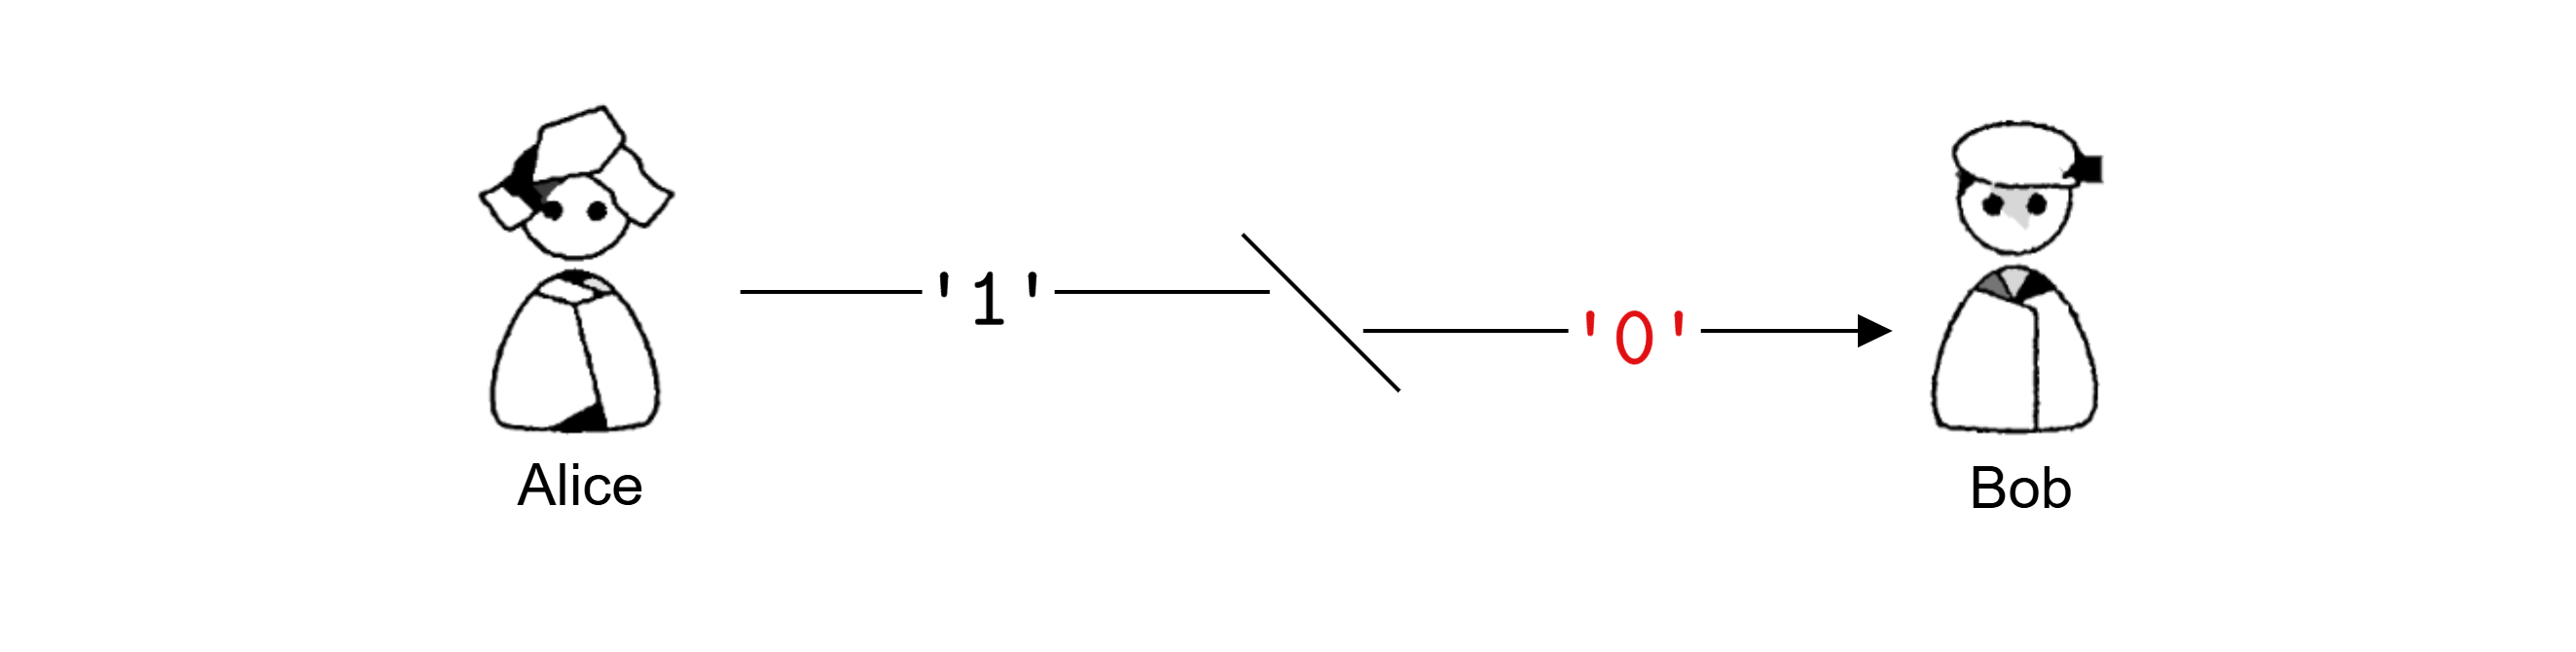
\includegraphics[width=\textwidth]{./Sections/comp/info_effic/noisy.png}
    \caption{Alice and Bob trying to communicate `1' for heads, but the message is corrupted, and Bob 
    receives a `0' instead. }
    \label{fig:error_detection}
\end{figure}

\noindent
As we see above, such a single bit error can be catastrophic. To mitigate this, our encodings must be more robust.
\begin{Def}[Hamming Distance]

    A \textbf{Hamming distance} is the number of bit positions in which two same length encodings differ. If 
    there is a single bit error, the Hamming distance is 1. If there is none, then the two encodings are identical.
\end{Def}

\begin{Example}[Hamming Distance]

    \noindent
    The Hamming distance between the encodings,
    \[
    \begin{array}{ccccccc}
    0 & 1 & \textcolor{red}{1} & 0 & 1 & 1 & \textcolor{red}{1} \\
    0 & 1 & \textcolor{red}{0} & 0 & 1 & 1 & \textcolor{red}{0} \\
    \end{array}
    \]
    \noindent
    is 2, as there are two bit positions that differ (marked in red).
\end{Example}

\newpage 

\noindent
\begin{Def}[Single-bit Error Detection]

    If two valid distinct encodings have a Hamming distance of 1, then a single-bit error may occur;
    Therefore if we increase the minimum Hamming distance to 2, we can detect single-bit errors. 
    This may be done by adding a parity bit to the end of the encoding:
    \begin{itemize}
        \item \textbf{Even Parity:} Once added, the total number of 1's in the encoding is even.
        \item \textbf{Odd Parity:} Once added, the total number of 1's in the encoding is odd.
    \end{itemize}

\end{Def}

\begin{figure}[ht!]
    \centering
    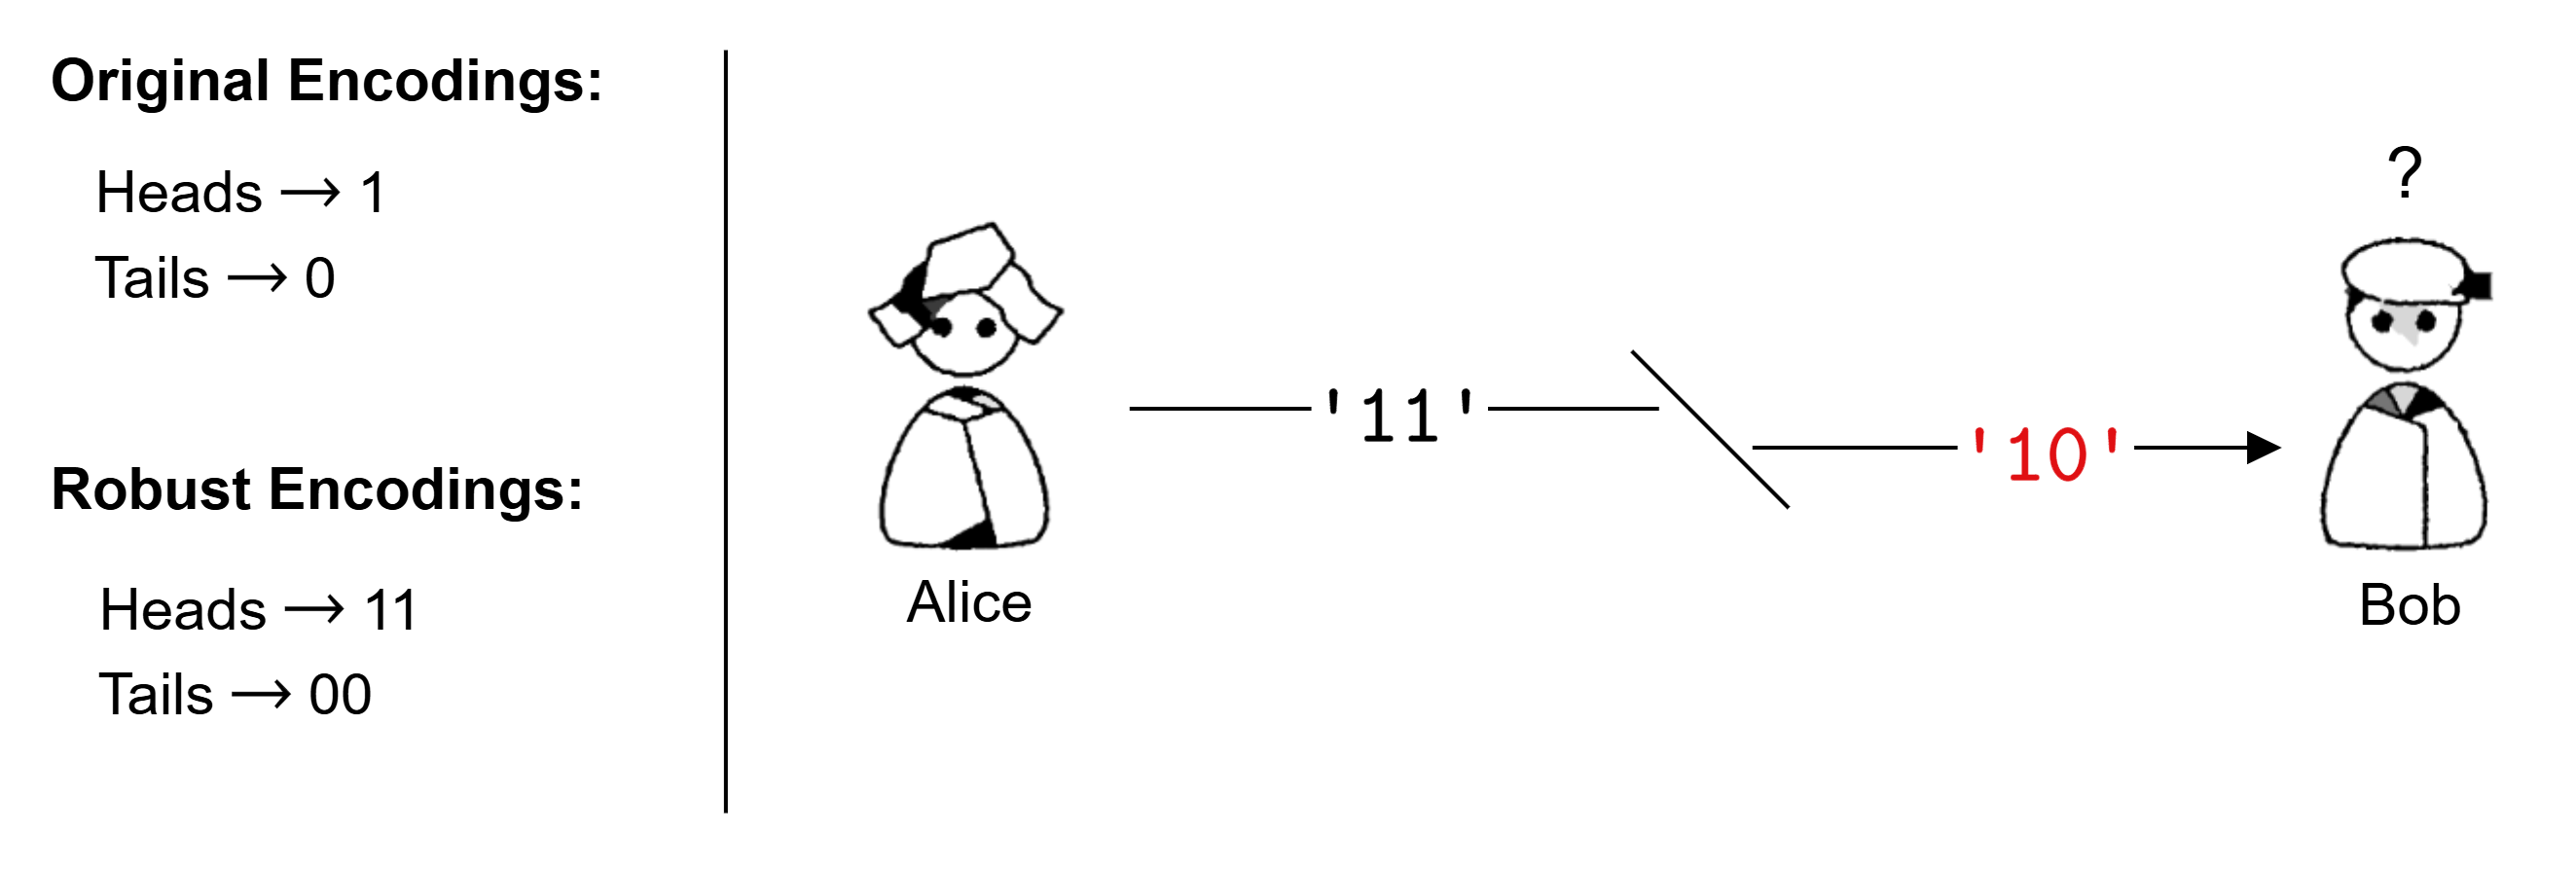
\includegraphics[width=\textwidth]{./Sections/comp/info_effic/parity.png}
    \caption{Alice and Bob using even parity to detect single-bit errors. Bob receives a single bit error and immediately detects it
    by checking the parity. \textbf{Note:} This does not help us if more than one bit is flipped.}
    \label{fig:parity}
\end{figure}

\begin{theo}[Detecting Multi-bit Errors]

    \label{theo:multi_bit_error_detection}  


    To detect $E$ errors within an encoding, a minimum Hamming distance of $E+1$ is required 
    between each code word. 
\end{theo}

\begin{theo}[Error Correction]

    \label{theo:error_correction}

    Let there be code $A$ and $B$, if the Hamming distance between them is $2E+1$, then we can correct $E$ errors.
    This is because the set of possible errors $A_e$ and $B_e$ will not overlap, allowing us to deduce the original encoding.
\end{theo}